%%%% This Beamer example was created by LianTze Lim, April 2017.

%%%% This is a VERY simple and minimalistic beamer theme,
%%%% even reminiscent of marker pens on transparencies!
%%%% It mimics the look of the "seminar" package, which
%%%% can only be used with plain TeX.
%%%% There are also some comments and example to show how
%%%% to customise various elements, e.g. the font and colours.

\documentclass[12pt, aspectratio=169]{beamer}
%% If you'd like the default font size to be even larger, use 14pt or 17pt; these are supported by Beamer.

\usepackage[english]{babel}
\usepackage[utf8]{inputenc}
\usepackage[T1]{fontenc}
\usepackage{lmodern}

%%%%%%%%%%%%%%%%%%%%%%%%%%%%%%%%%%%%%%%%%
% These lines should usually go into a .sty file,
% but I'll leave them here so that it's easier to
% see how to customise a Beamer theme.
% Remember, the Beamer manual is your friend!!
% http://texdoc.net/pkg/beamer
%
%% So if your re-definitions have a @ somewhere, you
%% _MUST_ put a \makeatletter before these lines and then
%% \makeatother after them. This trick can only be done
%% in the preamble! BUT if you're doing these re-definitions
%% in a .sty file (so that you \usepackage it later), you
%% don't need the \makeatletter and \makeatother.
\makeatletter

%% Set the left and right margins
\setbeamersize{text margin left=1em,text margin right=1em}

%% FONTS
\setbeamerfont{title}{series=\bfseries,size=\LARGE}
\setbeamerfont{subtitle}{series=\bfseries,size=\Large}
\setbeamerfont{frametitle}{series=\bfseries,size=\small}
\setbeamerfont{block title}{series=\bfseries,size=\normalsize}
\setbeamerfont{footline}{size=\normalsize}

%% COLOURS
%% If you'd like everything to have the same colour
%%\usebeamercolor{structure}

%% Add a line after the frametitle
\addtobeamertemplate{frametitle}{}{\vspace*{-1ex}\rule{\textwidth}{1pt}}

%% Use circular discs as itemized list markers;
%% there's an existing option in Beamer for it so I'll use it
\setbeamertemplate{itemize items}[circle]

%% Remove default navigation symbols (We'll add the ones we need in the footline
\setbeamertemplate{navigation symbols}{}


%% And before the footline... actually we'd like to re-define
%% the footline
\setbeamertemplate{footline}{%
   %% Beamer headlines and footlines are always full-paperwidth, so if you want the horizontal line to
   %% not span it entirely you'll need to do a bit of arithmetic
   \centering
   \begin{minipage}{\dimexpr\paperwidth-\beamer@leftmargin-\beamer@rightmargin\relax}
   \centering
   \rule{\linewidth}{1pt}\vskip2pt
   \usebeamerfont{footline}%
   \usebeamercolor{footline}%
   %% The frame number smack in the middle
   \hfill\insertpagenumber/\inserttotalframenumber
   \hfill%
   %% ONLY the navigation symbols we want at the far right.
   %% We use an \llap so that it takes up zero width, and doesn't throw the page number off-centre!
   \llap{\insertframenavigationsymbol\insertbackfindforwardnavigationsymbol}\par
   \end{minipage}\vskip2pt
}

\makeatother
%%%% END STYLE CUSTOMISATION %%%%%%%%%%%%



\title{Statistics}
\subtitle{How do we know?}
\author{Elisea Jackson}
\date{April 2017}

\begin{document}

\begin{frame}
  \titlepage
\end{frame}

% Uncomment these lines for an automatically generated outline.
%\begin{frame}{Outline}
%  \tableofcontents
%\end{frame}

\section{Introduction}

\begin{frame}{Creation of Statistics}

\begin{itemize}
  \item collection
  \item organization
  \item analization
  \item interpretation
  \item presentation
\end{itemize}
\end{frame}

\begin{frame}{Mathematical Statistics}
  The use of mathmatical equations and probability to collect data, in place of collecting data. Started with disscusions of games of chance. 
  There is a lot!!!
\end{frame}


\begin{frame}{Monte Carlo}
  Normal Distribution Function / Gaussian Distribution
  \begin{columns}
    \column{0.5\linewidth}
    \centering
    \begin{figure}
      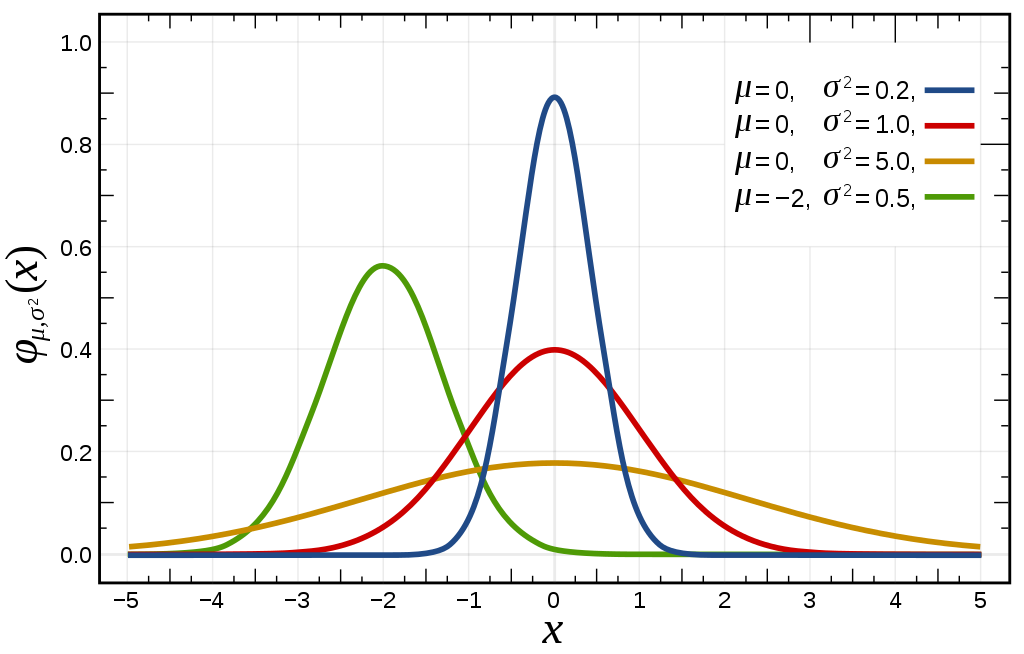
\includegraphics[width=\textwidth]{1024px-norm.png}
    \end{figure}
    Probability Density Function
    \column{0.5\linewidth}
    \centering
    \begin{figure}
      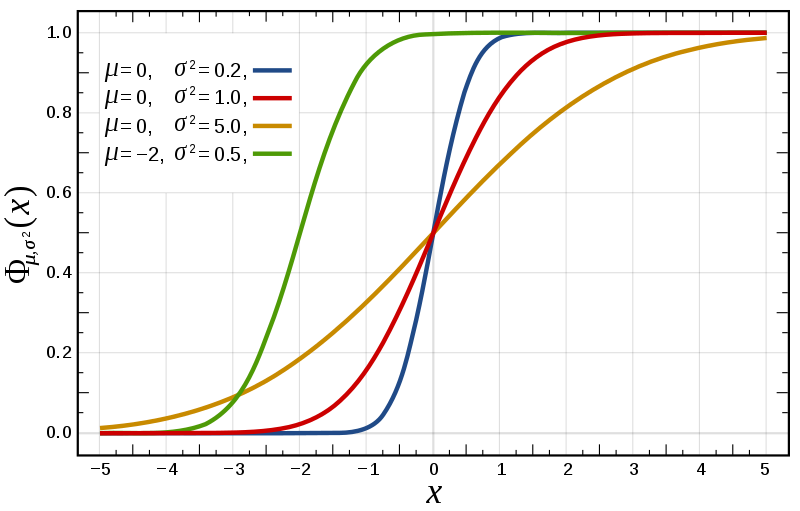
\includegraphics[width=\textwidth]{800px-dist.png}
    \end{figure}
    Cumulative Distribution Function
  \end{columns}
\end{frame}


\begin{frame}{Poission Distribution}
Each event happens sepate from the last and they share a common mean. 
% Commands to include a figure:
             \centering
               \begin{figure}
                 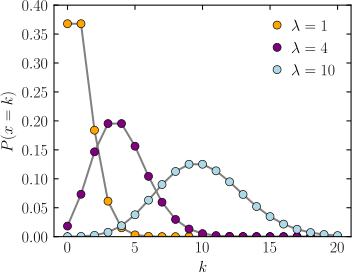
\includegraphics[width=0.5\textwidth]{Poisson_pmf.svg.png}
               \end{figure}


\end{frame}


\begin{frame}{Random Correlations}
  \centering
  \begin{figure}
    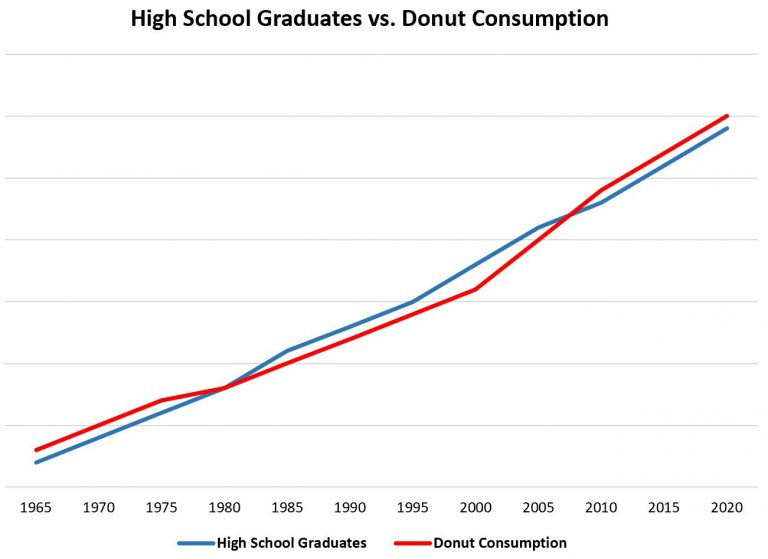
\includegraphics[width=0.6\textwidth]{correlation3.jpg}
  \end{figure}

            
\end{frame}

\begin{frame}{Random Correlations}
  \centering
  \begin{figure}
    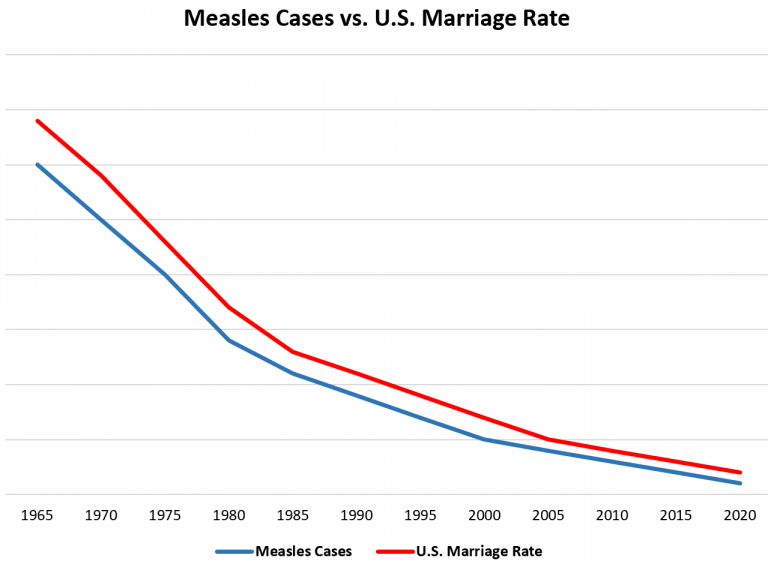
\includegraphics[width=0.6\textwidth]{correlations2.png}
  \end{figure}

            
\end{frame}

\begin{frame}{Random Correlations}
  \centering
  \begin{figure}
    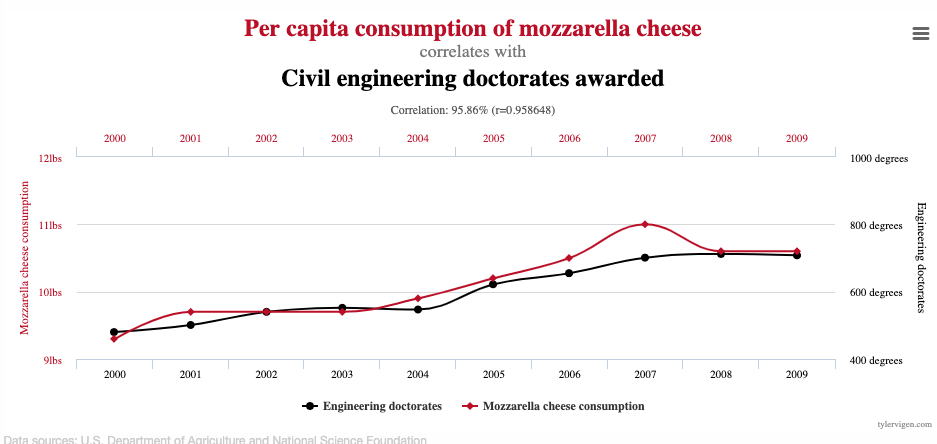
\includegraphics[width=0.75\textwidth]{correlations1.png}
  \end{figure}

            
\end{frame}




\end{document}
